\begin{figure}
  \centering
  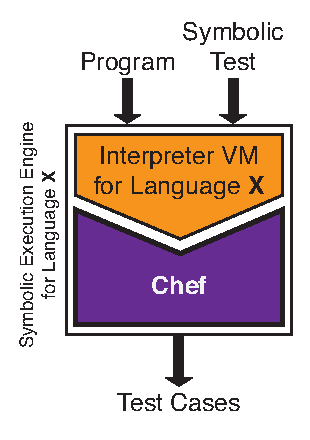
\includegraphics[width=0.3\textwidth]{chef/figures/usage-model}
  \caption{Overview of \chef's usage.}
  \label{fig:chef:overview}
\end{figure}

\chef is a platform for language-specific symbolic execution.
%
Provided with an interpreter environment, which acts as an executable language specification, \chef becomes a symbolic execution engine for the target language (see Figure~\ref{fig:chef:overview}).
%
The resulting engine can be used like a hand-written one, in particular for test case generation.  When supplied with a target program and a symbolic test case (also called test driver or test specification in the literature), the \chef engine outputs a set of concrete test cases, as shown in Figure~\ref{fig:chef:overview}.

\paragraph{Example}

\begin{figure}
  \centering
  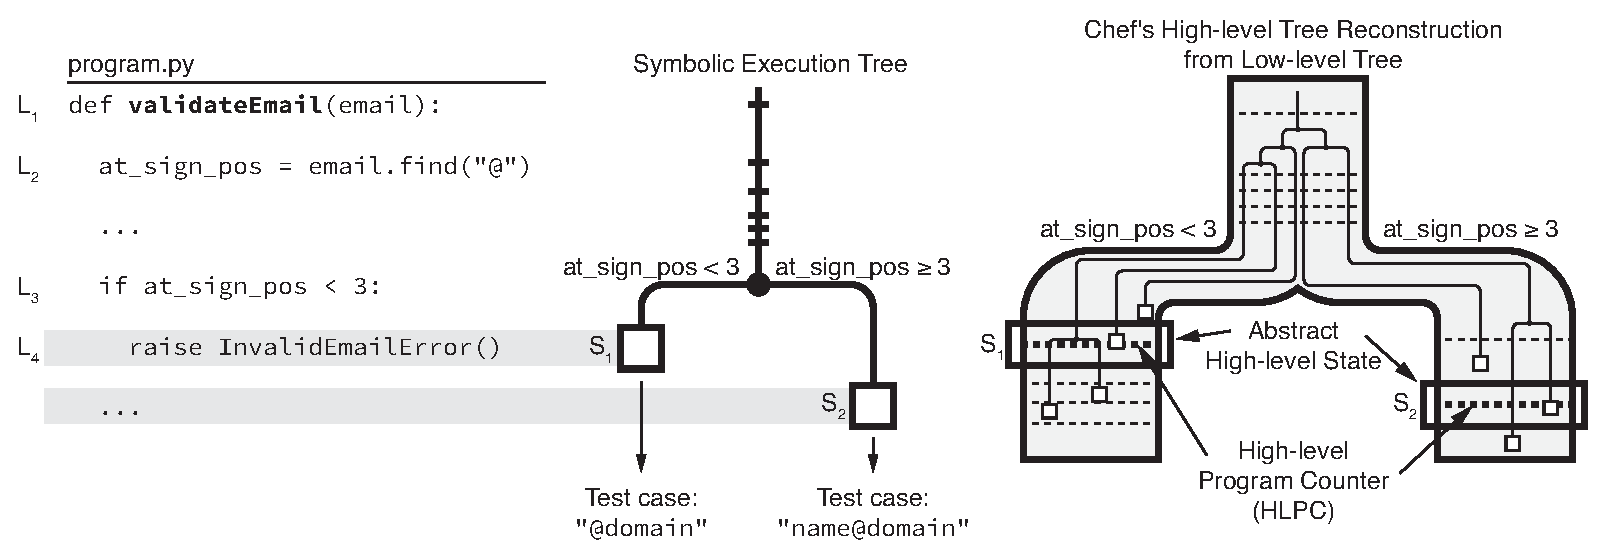
\includegraphics[width=\textwidth]{chef/figures/running-example}
  \caption[Example of Python code that validates an e-mail address given as a string with corresponding symbolic execution tree and mapping of interpreter paths to program paths.]{Example of Python code that validates an e-mail address given as a string (left) with corresponding symbolic execution tree (center) and mapping of interpreter paths to program paths (right).  Marks on the execution path indicate program statements.}
  \label{fig:chef:running-example}
\end{figure}

We illustrate the functionality of \chef using the Python example in Figure~\ref{fig:chef:running-example} (left).
%
The function \codebit{validateEmail} receives an e-mail address string and raises an exception if the address is malformed.
%
We symbolically execute the function using a \chef engine obtained by plugging in it the Python interpreter.

The \chef engine receives the Python program together with a symbolic test that marks the \codebit{email} input argument as symbolic.

\chef constructs the symbolic execution tree of the program, as shown in Figure~\ref{fig:chef:running-example} (center).
%
The paths in the tree are sequences of program locations, corresponding to a statement or bytecode instruction.  Branches can occur explicitly at control flow statements (as in our example), or implicitly through exceptions.

\chef prioritizes execution states according to a pluggable search strategy (see Section~\ref{sec:intro:symbex}).
%
There are two execution states in our example: $S_1$, which executes the exception path, and $S_2$, which executes the normal path.
%
A strategy may randomly select states to uniformly cover the set of possible paths, or it may favor the states that are triggering exceptions in the program, such as $S_1$.

At the end of each execution path, \chef generates a concrete string value for the \codebit{email} argument, which constitutes a test case.
%
Each test case takes the Python program along the same execution path, when replayed in the same interpreter.


\paragraph{The Interpreter as Language Specification}

\chef is built on top of the S2E analysis platform~\cite{s2eSystem}, which symbolically executes the interpreter environment \emph{at binary level}.
%
The interpreter environment is a virtual machine that bundles the interpreter, a testing library, the operating system, and other user programs.
%
For example, to symbolically execute the program in Figure~\ref{fig:chef:running-example},  \chef runs the interpreter by invoking \codebit{./python program.py} inside the virtual machine.

The resulting engine is a correct symbolic execution engine for the target language \emph{as defined by the interpreter}.
%
It is fully precise and theoretically complete, i.e., it will not explore infeasible paths and will eventually explore all paths.\footnote{The usual limitations of symbolic execution engines apply: completeness holds only under the assumption that the constraint solver can reason about all generated path conditions, and it is understood that exhaustive exploration is usually impractical in finite time.}

%%% Local Variables: 
%%% mode: latex
%%% eval: (visual-line-mode)
%%% fill-column: 1000000
%%% TeX-master: "main"
%%% End:
